\documentclass[twocolumn,showkeys,preprintnumbers,amsmath,amssymb]{revtex4}
\usepackage{graphicx}
\usepackage{caption}
\usepackage{subcaption}
\captionsetup{compatibility=false}
\usepackage{dcolumn}
\usepackage{bm}
\usepackage[utf8]{inputenc}
\usepackage[spanish]{babel}
\usepackage{multirow}
\usepackage{float}
\usepackage{url}
\usepackage[decimalsymbol=point]{siunitx}
\sisetup{output-exponent-marker=\ensuremath{\mathrm{e}}}
\decimalpoint
\usepackage{array}
\providecommand{\e}[1]{\ensuremath{\times 10^{#1}}}

\begin{document}

\preprint{}

\title{Informe 4: Efecto Hall}

\author{Iván Mauricio Burbano}
\email{im.burbano10@uniandes.edu.co}
\author{Juan David Castillo}
 \email{jd.castillo10@uniandes.edu.co}
\affiliation{Universidad de los Andes \\ Departamento de Física}

\date{\today}

\begin{abstract}
	
En este experimento se explora el efecto Hall en dos muestras de germanio dopadas tipo n y tipo p. Se determina el coeficiente de Hall de las muestras mediante mediciones a campo magnético constante y mediciones a corriente constante. Se concluye que el método que entrega mejores resultados es el de campo magnético constante. También se mide una resistencia de $37\Omega$ y $48\Omega$ para la muestra tipo n y tipo p sin campo. Se observo el fenómeno de magnetoresistencia y se hizo un ajuste experimental cuadrático para la relación entre resistencia y campo magnético. Se confirmaron mediciones previas de Purwar\cite{bib:Purwar} de disminución de resistencia en presencia de campo magnéticos bajos. Se evidenció la utilidad de la técnica de dopaje de semiconductores al medir una disminución del gap de energía del Germanio dopado tipo n con respecto al gap de energía del Germanio intrínseco reportado en la literatura\cite{bib:Ge}.
	
\end{abstract}

\keywords{efecto Hall, semiconductores, dopaje tipo n y tipo p, gap de energía, ley de Ohm.}

\maketitle

\section{\label{sec:int} Introducción}

	En este experimento se va a trabajar con el Germanio. Este elemento qu\'imico tiene un n\'umero at\'omico de 32, por lo que en su estado neutro tiene 4 electrones en el nivel de energ\'ia de valencia. Entre la banda de valencia y la banda de conducci\'on, el germanio tiene un \textit{gap} de energ\'ia de tan solo $0.661eV$\cite{bib:Ge}. Este gap tan peque\~no permite que debido a excitaciones t\'ermicas, algunos de los electrones en la banda de valencia pueden subir a la banda de conducci\'on, actuando como portadores para el paso de corriente y dejando huecos en la banda de valencia. Para aumentar la cantidad de portadores en el Germanio es com\'un agregar impurezas. Si se agregan As, P, Sb, Bi o Li se adicionan electrones y se logra un dopaje tipo n como muestra la figura \ref{fig:tipon}. De manera similar, agregar Al, B, Ga, In o Tl, produce un d\'eficit de electrones (estos materiales solo tienen tres electrones en su \'ultimo nivel de energ\'ia), es decir, a\~nade huecos al sistema.

	\begin{figure}
		\centering
		\caption{Se muestra como la adici\'on de una impureza en una red de Germanio puede a\~nadir portadores al sistema para facilitar la conducci\'on\cite{bib:tipon}.}
		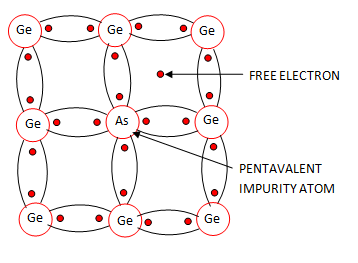
\includegraphics[width=0.45\textwidth]{tipon.png}
		\label{fig:tipon}
	\end{figure}

	Ahora suponga que se tiene una l\'amina de Ge como la que se muestra en la figura \ref{fig:lamina}. En el caso estacionario se van a asumir que fluyen portadores de carga $q$ en la direcci\'on del eje $x$ con velocidad $v$ constante. Para evitar el flujo de portadores en la direcci\'on de $y$ es necesario que se produzca un campo el\'ectrico en esta de valor $E_y=vB$ donde $B$ es el campo magn\'etico aplicado en la direcci\'on $z$. Este campo inducido genera lo que se conoce como el voltaje de Hall $V_H$ (el m\'odulo de l potencial inducido) y permite definir el coeficiente de Hall como $R_H=E_y/jB$ donde $j$ es la densidad de corriente. Si se detecta una corriente $I$ que fluye por la l\'amina y un voltaje de hall $V_H$ en la direcci\'on de la figura, se tiene $R_H=\frac{V_H/d}{BI/wd}=\frac{V_Hw}{IB}$. Note que esta expresi\'on solo es valida para huecos pues $V_H$ es definido positivo y se utiliz\'o $E_y=V_H/d$. Para electrones se tiene que $R_H=\frac{-V_Hw}{IB}$. Tomando $I$ y $V_H$ como las variables dependiente e independiente respectivamente, llegamos a la ecuación:
	
	\begin{equation}
		V_H=\pm \frac{R_H B}{w} I \label{eq:RH}
	\end{equation}
	
	Que será utilizada para encontrar $R_H$.

	\begin{figure}
		\centering
		\caption{Se muestra el sistema de coordenadas que se va a utilizar durante el informe con respecto a la l\'amina de Ge\cite{bib:guia}.}
		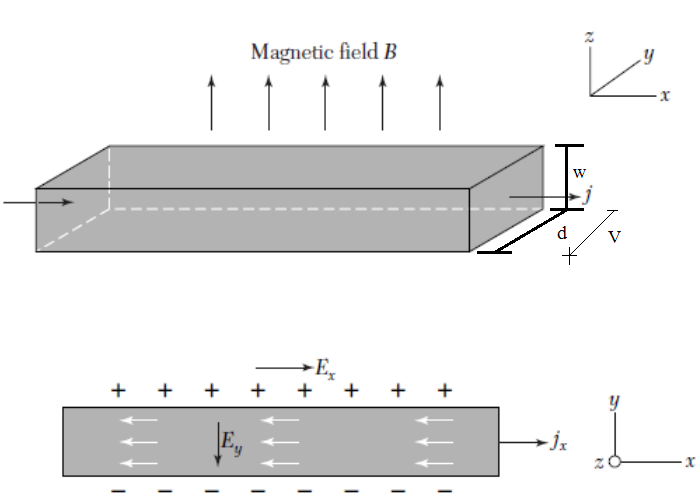
\includegraphics[width=0.45\textwidth]{hall.png}
		\label{fig:lamina}
	\end{figure}

	El coeficiente de Hall nos permite determinar la densidad de los portadores. Si se tiene una densidad de huecos $n_h$ y de electrones $n_e$, con velocidades $v_{hy}$ y $v_{ey}$ en la direcci\'on $y$ respectivamente, se tiene que la densidad de corriente en $y$ es $n_hev_{hy}-n_eev_{ey}$. Imponiendo que no haya un transporte de carga en esta direcci\'on y utilizando la f\'ormula de fuerza de Lorentz, podemos hallar el campo el\'ectrico inducido en $y$. Este procedimiento nos permite calcular el coeficiente de Hall en t\'erminos de los portadores como

	\begin{equation} \label{eq:rhcomplicado}
		R_H=\frac{n_h\mu_h^2-n_e\mu_e^2}{e(n_e\mu_e+n_h\mu_h)^2}
	\end{equation}

	donde $\mu_h$ y $\mu_e$ son los coeficientes de movilidad de los huecos y los electrones respectivamente.
	
	La conductividad y el valor de $r_H$ en el germanio también se ven afectados por la temperatura de la muestra en cuestión. Cuando el germanio se encuentra en la región de conducción intrínseca, la conductividad cambia con la temperatura de acuerdo a la ecuación
	
	\begin{equation}
		\sigma = \sigma_0 e^{\frac{E_g}{\kappa_B T}} \label{eq:CondTemp}
	\end{equation}
	
	
	
	

\section{\label{sec:mont} Montaje Experimental}

	\subsection*{Equipo}

		\begin{itemize}
	
			\item Módulo de efecto Hall
	
			\item Tarjetas de efecto Hall: p-Ge y n-Ge, con sensores de temperatura.
	
			\item Multímetro X 3
		
			\item Teslámetro
	
			\item Fuentes de poder AC y DC
	
			\item Electroimán
	
			\item Soporte
	
			\item Cables
	
	\end{itemize}

	Primero, se montó el módulo Hall con una de las tarjetas y se colocó el semiconductor con cuidado en el camino del electroimán. Se conectó el electroimán a la fuente DC y se utilizó el Teslámetro para poder establecer una correlación lineal entre la magnitud de la corriente y la intensidad de campo magnético, para poder convertir todos los datos de corriente DC obtenidos en datos de campo magnético.

	Después, se aplicó al semiconductor un campo magnético constante y se midió el voltaje de Hall en función de la corriente aplicada al semiconductor. Se repitió esta medición varias veces repitiendo campos magnéticos, y se hizo esto para cada tarjeta, para observar los efectos del dopaje en los datos.

	Después, se dejó la corriente de la muestra constante y se efectuaron mediciones de voltaje en función del campo magnético. Teóricamente deberian obtenerse resultados similares para el valor de $R_H$. Se hizo una medición adicional de este tipo pero invirtiendo la dirección del campo magnético, para comprobar la simetría del sistema.

	Ahora, se medirá la resistencia de cada tarjeta en función de la temperatura. Para hacer esto, se midió la caída de voltaje en función de la corriente, para obtener la pendiente de valor $R_0$. Después, se midió el cambio de resistencia en función de la intensidad de campo magnético para una corriente constante. Finalmente, se midió la caída de voltaje de la muestra y el voltaje de Hall para una corriente constante y campo magnético constante, pero variando la temperatura del semiconductor.
	


\section{\label{sec:resu} Resultados y Análisis}
	
	\subsection{Campo magnético en función de la corriente}
	
		Utilizando el Teslámetro, se midió el campo magnético en función de la corriente tanto con la tarjeta dentro del montaje como al aire libre, con los siguientes resultados:
		
		\begin{figure}[H]
			\centering
			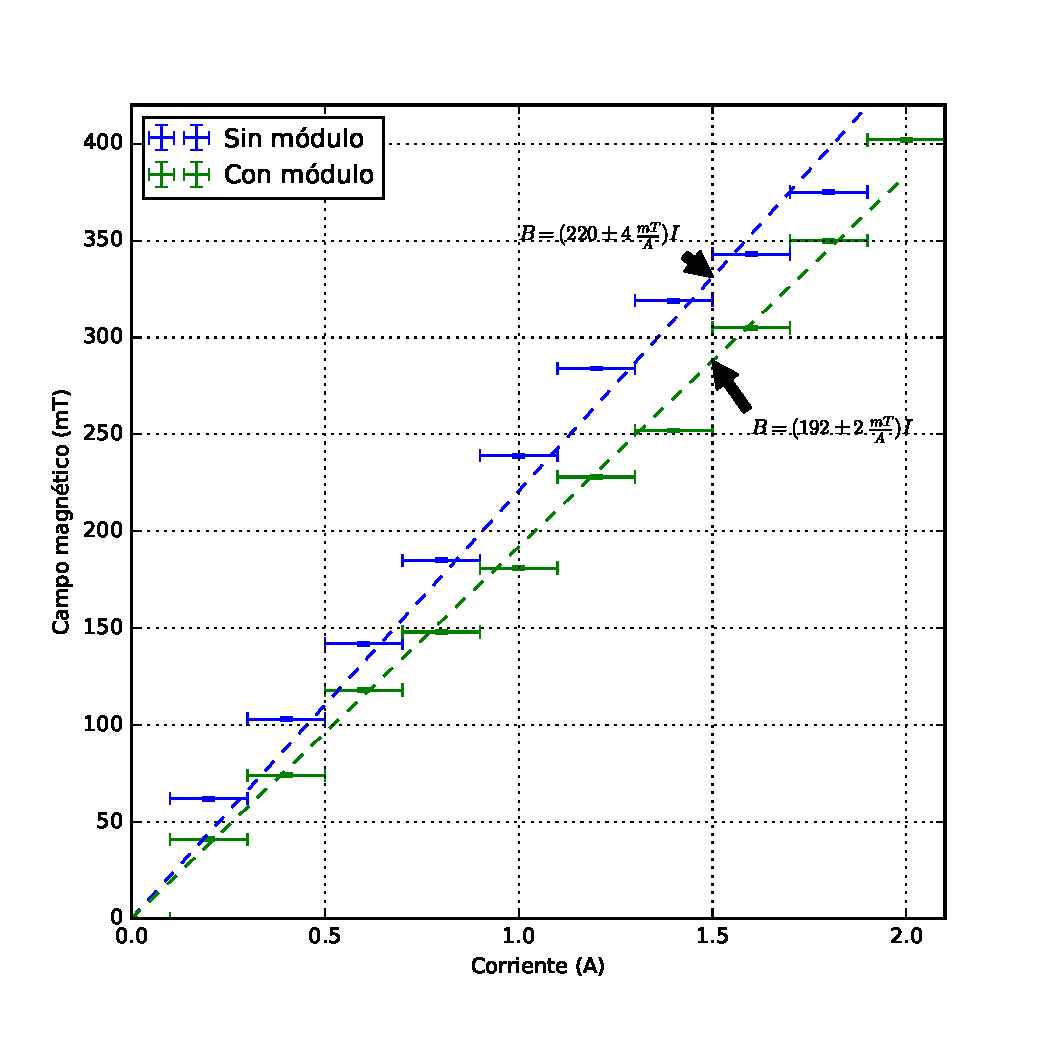
\includegraphics[width=0.45\textwidth]{B.pdf}
			\caption{Campo magnético en función de la corriente}
			\label{tab:b}
		\end{figure}
		
		Debido a que las mediciones con el módulo puesto son más parecidas a los casos que se medirán en las siguientes tomas, se utilizará esta relación ($192\pm 2 \frac{mT}{A}I$) para convertir datos de corriente en las bobinas en datos de campo magnético a través de la tarjeta,.
		
	\subsection{\label{subsec:VHallIConst} Voltaje de Hall en función de la corriente para un campo fijo.}
	
		Para distintas intensidades de campo magnético, se tomaron valores de voltaje de Hall en función de la corriente a través del semiconductor utilizado, para los semiconductores de tipo $n$ y $p$. Estas mediciones arrojaron los datos que se presentan en las siguientes tablas:
		
		\begin{widetext}
			
			\begin{figure}[H]
				\centering
				\begin{subfigure}[b]{0.45\textwidth}
					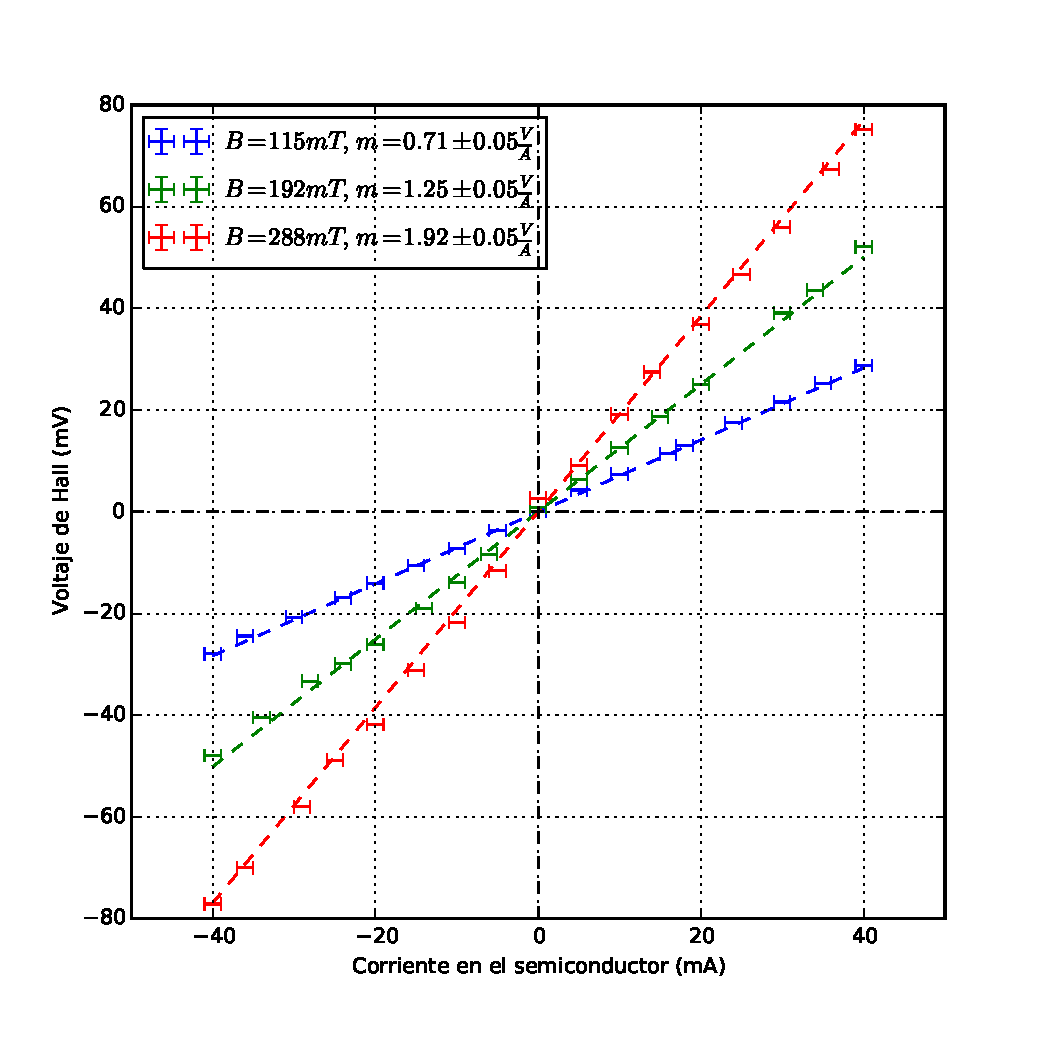
\includegraphics[width=\textwidth]{BConst-NGe.pdf}
					\caption{Germanio tipo n.}
					\label{fig:BConst-NGe}
				\end{subfigure}
				\begin{subfigure}[b]{0.45\textwidth}
					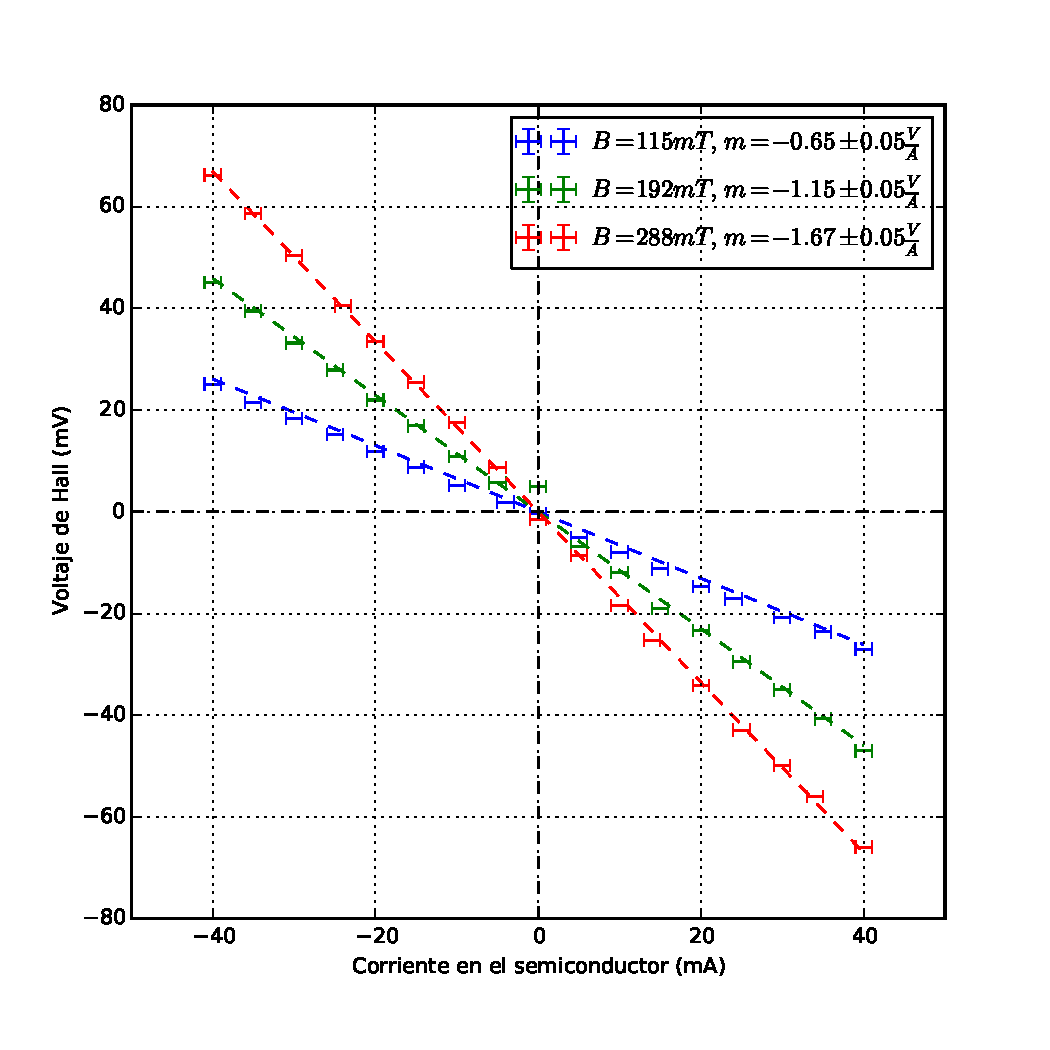
\includegraphics[width=\textwidth]{BConst-PGe.pdf}
					\caption{Germanio tipo p.}
					\label{fig:BConst-PGe}
				\end{subfigure}
				\caption{$V_{hall}$ en función de la corriente para campos magnéticos constantes}
				\label{fig:BConst}
			\end{figure}
			
		\end{widetext}
		
		Cualitativamente se puede observar que debe haber un error, ya que según la literatura las pendientes del germanio tipo $n$ deberían ser negativas y las del $p$ positivas. Por lo tanto, es evidente que las bobinas del inductor fueron conectadas al revés y se obtuvo un campo magnético con un signo opuesto al asumido. Entonces, para poder aprovechar todas las otras mediciones efectuadas, se asumirá que el montaje produce resultados simétricos y que los resultados obtenidos serían idénticos pero con los signos opuestos si se invierten los valores de campo magnético.
		
		En base a esta suposición, y utilizando las ecuación \eqref{eq:RH} para un valor de $w$ reportado de $1\times 10^{-3}m$\cite{bib:guia}, se obtuvieron los siguientes datos de las regresiones lineales efectuadas:
		
		\begin{table}[H]
			\centering
			\begin{tabular}{ c | c | c | c }
				Semiconductor & $B$ & $\frac{R_H B}{w}$ & $R_H \ \left( 10^{-3}\frac{m^3}{C} \right)$ \\
				& (mT) & $\left(\frac{V}{A} \pm 0.05 \frac{V}{A} \right)$ & \\ \hline
				\multirow{3}{*}{n-Ge} & $115 \pm 1$ & -0.71 & $-6.2\pm 0.8$ \\
				 & $192 \pm 2$ & -1.25 & $-6.5\pm 0.4$ \\
				 & $288 \pm 2$ & -1.92 & $-6.7\pm 0.3$ \\ \hline
				\multirow{3}{*}{p-Ge} & $115 \pm 1$ & 0.65 & $5.6\pm 0.8$ \\
				 & $192 \pm 2$ & 1.15 & $6.0\pm 0.4$ \\
				 & $288 \pm 2$ & 1.67 & $5.8\pm 0.3$ \\
			\end{tabular}
			\caption{Datos de $R_H$ obtenidos para cada semiconductor en las mediciones}
			\label{tab:RH-BConst}
		\end{table}
		
	\subsection{Voltaje de Hall en función del campo magnético para una corriente fija}
		
		Esta toma es similar a la anterior, pero se dejó la corriente a través del semiconductor como una constante y se permitió que el campo magnético fuera variable. Se efectuó una toma con el campo magnético invertido. Haciendo uso de la ecuación \eqref{eq:RH}, se obtiene una regresión lineal para valores de $\frac{R_H I}{w}$. Los datos obtenidos en esta toma fueron:
		
		\begin{widetext}
			
			\begin{figure}[H]
				\centering
				\begin{subfigure}[b]{0.45\textwidth}
					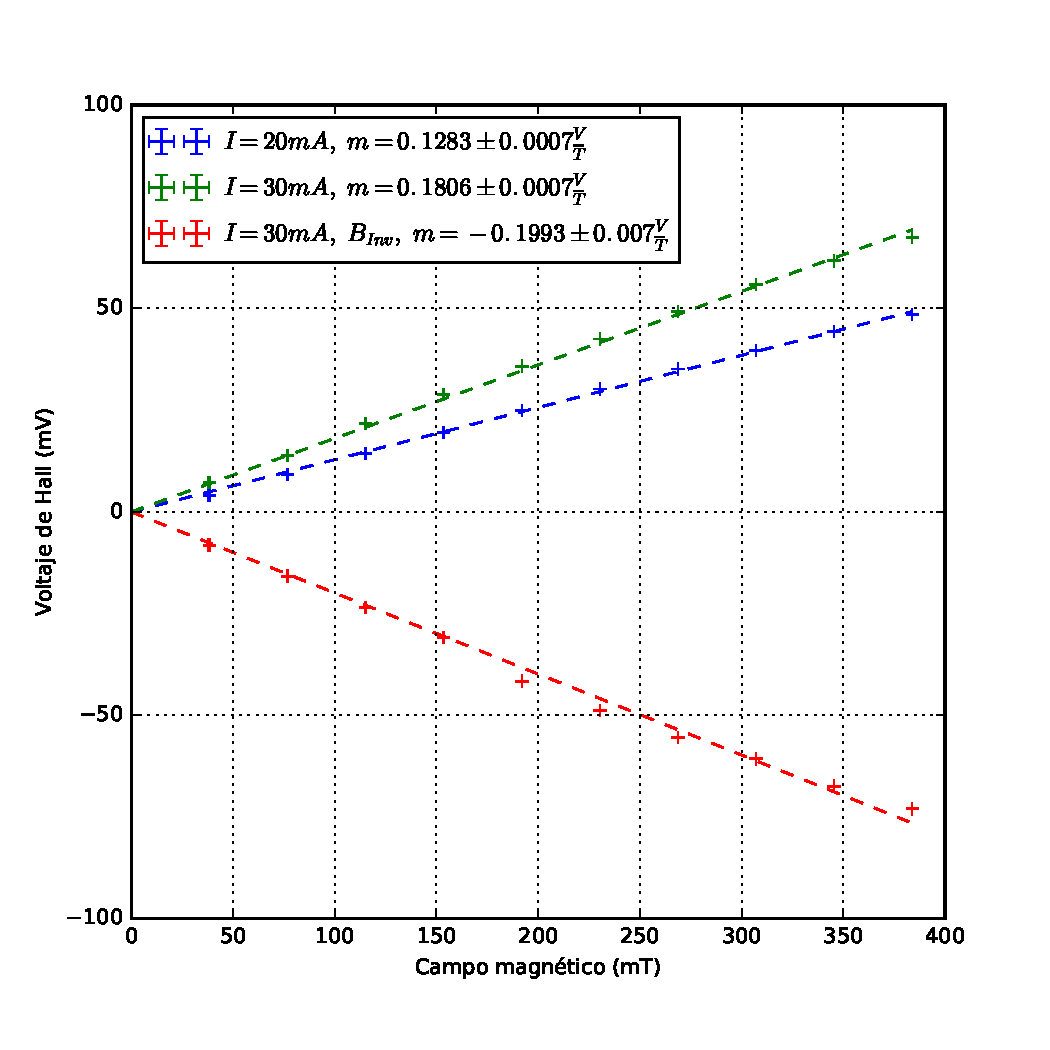
\includegraphics[width=\textwidth]{IConst-NGe.pdf}
					\caption{Germanio tipo n.}
					\label{fig:IConst-NGe}
				\end{subfigure}
				\begin{subfigure}[b]{0.45\textwidth}
					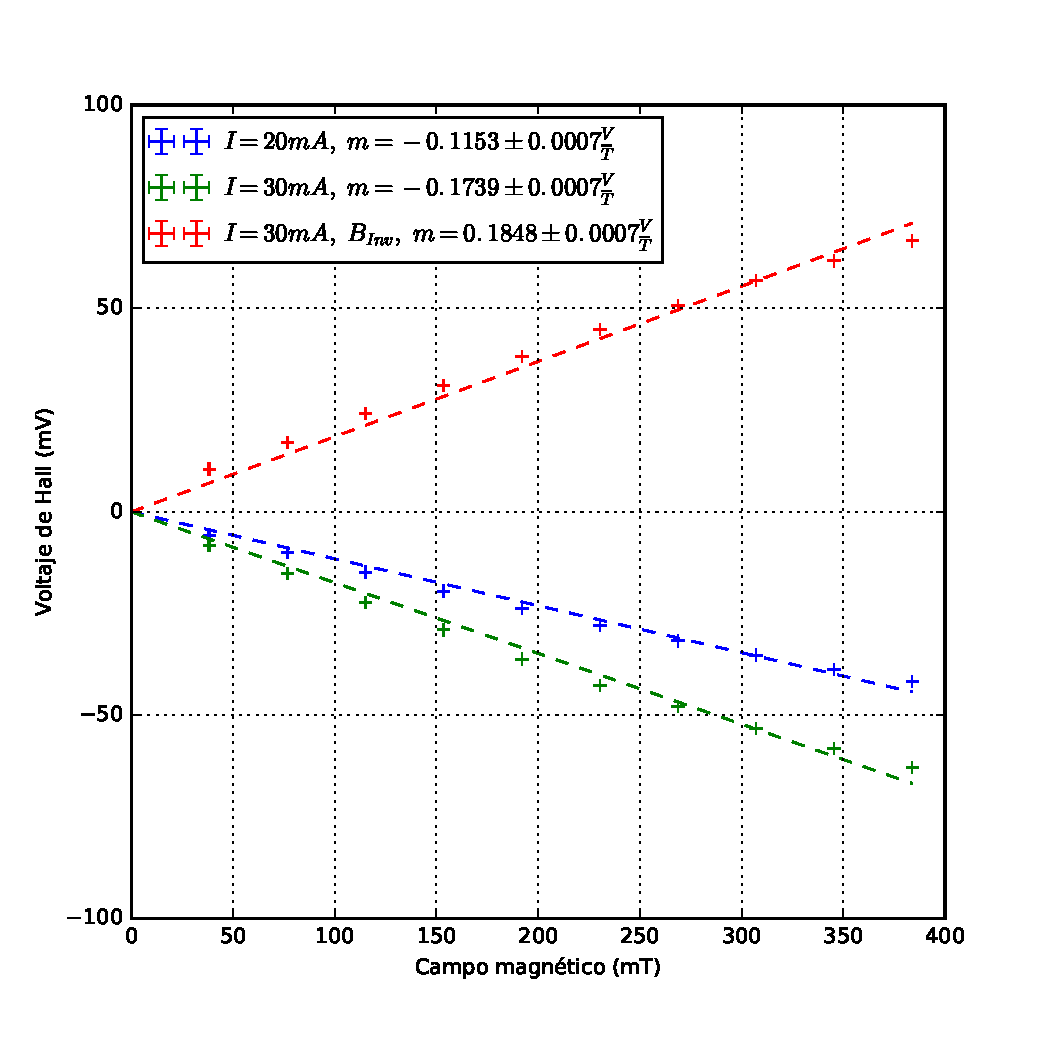
\includegraphics[width=\textwidth]{IConst-PGe.pdf}
					\caption{Germanio tipo p.}
					\label{fig:IConst-PGe}
				\end{subfigure}
				\caption{$V_{hall}$ en función del campo magnético para corrientes constantes}
				\label{fig:IConst}
			\end{figure}
			
		\end{widetext}
		
		En base a esto, y teniendo en cuenta la corrección de signos que se hizo en el ejercicio pasado se obtuvieron los siguientes valores de $R_H$ para ambos materiales:
		
		\begin{table}[H]
			\centering
			\begin{tabular}{ c | c | c | c }
				Semiconductor & $I$ & $\frac{R_H I}{w}$ & $R_H \ \left( 10^{-3}\frac{m^3}{C} \right)$ \\
				& (mA) & $\left(\frac{V}{mT} \pm 7 \e{-4} \frac{V}{mT} \right)$ & \\ \hline
				\multirow{3}{*}{n-Ge} & 20 & -0.1283 & $-6.41\pm 0.09$ \\
				& 30 & -0.1806 & $-6.02\pm 0.08$ \\
				& 30 & 0.1993 & $6.64\pm 0.08$ \\ \hline
				\multirow{3}{*}{p-Ge} & 20 & 0.1153 & $5.77\pm 0.09$ \\
				& 30 & 0.1739 & $5.80\pm 0.08$ \\
				& 30 & -0.1848 & $-6.16\pm 0.08$ \\
			\end{tabular}
			\caption{Datos de $R_H$ obtenidos para cada semiconductor en las mediciones de corriente constante.}
			\label{tab:RH-IConst}
		\end{table}
		
	En primer lugar note que el cambio de dirección del campo magnético tiene el efecto esperado según la ecuación \eqref{eq:RH}. El signo de $R_H$ cambia ya que si antes los portadores se acumulaban en un borde de la muestra, con el campo magnético nuevo la fuerza de Lorentz cambia de signo y hace que los portadores se acumulen en el lado opuesto. El efecto neto de esto es cambiar la dirección del voltaje de Hall producido más no su magnitud, explicando el cambio en el signo de $R_H$ sin cambio de magnitud. 
	
	Como se explica en la sección \ref{sec:int}, el signo de los $R_H$ calculados nos permite deducir los portadores dentro del material. Como se esperaba, se puede concluir que la placa tipo n tiene como portadores electrones y la placa tipo p tiene como portadores huecos. Estos portadores por supuesto son extrínsecos ya que vienen del dopaje del Ge puro. Es gracias a este dopaje que dos muestras de Ge tienen un comportamiento tan distinto. 
	
	La exactitud de los resultados de $R_H$ no se pueden determinar por su valor ya que dependen fuertemente del dopaje individual de cada muestra y por lo tanto no se puede comparar con los valores hallados en \cite{bib:soporteN} y por eso no se entrega un valor promedio de los resultados obtenidos en las tablas \ref{tab:RH-BConst} y \ref{tab:RH-IConst}. Por el otro lado, si se puede evaluar la exactitud de los resultados mediante la comparación entre ellos. Se puede apreciar que la determinación de $R_H$ con campo magnético constante es mejor que con corriente constante. En el primer caso todos los resultados se encuentran dentro de las tolerancias encontradas a partir de la regresión lineal. En el segundo caso, si bien las regresiones lineales reportan un valor menos tolerante de $R_H$, las aproximaciones utilizadas para llegar a $R_H$ constante dejan de ser validas. En particular, permitir la variación de campo magnético produce la variación del gradiente de temperatura mediante el fenómeno de Righi-Leduc. Esta alteración en el gradiente de temperatura que no se tuvo en cuenta en el análisis de la sección \ref{sec:int} altera la distribución energética espacial haciendo menos probable que los portadores se encuentren en los extremos de la muestra reduciendo así el voltaje Hall. Esta es una de las posibles causas de las discrepancias de los resultados en la tabla \ref{tab:RH-IConst}.
	
	Vale la pena comentar que en ningún momento se ha contemplado la posibilidad de que el dopaje sea mixto y se tenga que hacer un análisis con la ecuación \eqref{eq:rhcomplicado}.  		
		
	\subsection{Resistencia de los semiconductores sin campo magnético}
	
		Para determinar la resistencia de los semiconductores, se tomaron datos de voltaje en función de la corriente, con el siguiente resultado:
		
		\begin{figure}[H]
			\centering
			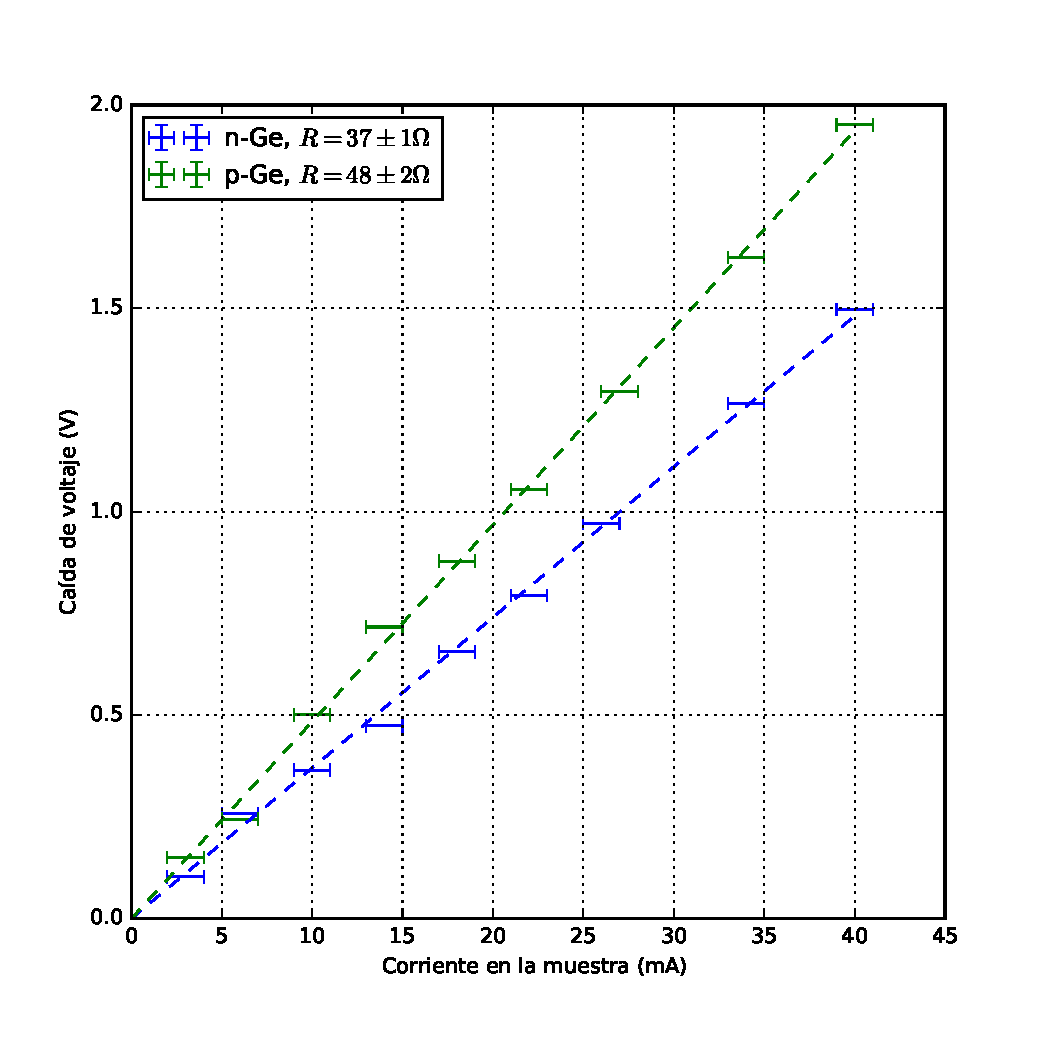
\includegraphics[width=0.45\textwidth]{RSinCampo.pdf}
			\caption{Líneas de voltaje en función de la corriente para ambas muestras}
			\label{fig:RSinCampo}
		\end{figure}
		
		Como se puede ver, el germanio dopado actúa como una resistencia lineal, por lo que se comporta de acuerdo a la ley de Ohm. el germanio tipo n posee una resistencia a temperatura ambiente de 37 Ohms, mientras que su equivalente tipo P tiene una resistencua de 48 Ohms. la magnitud de los errores absolutos se debe a la baja resolución del medidor de corriente a través de la muestra, que nos da las barras de error observadas en la dirección $x$.
		
	\subsection{Cambio de resistencia en los semiconductores por un campo magnético}
	
		El cambio en la resistencia se calculó midiendo el cambio en voltaje longitudinal en función del campo magnético para una corriente fija a través de la muestra. Transformando los datos obtenidos a datos de resistencia, se obtuvieron las siguientes curvas:
		
		\begin{figure}[H]
			\centering
			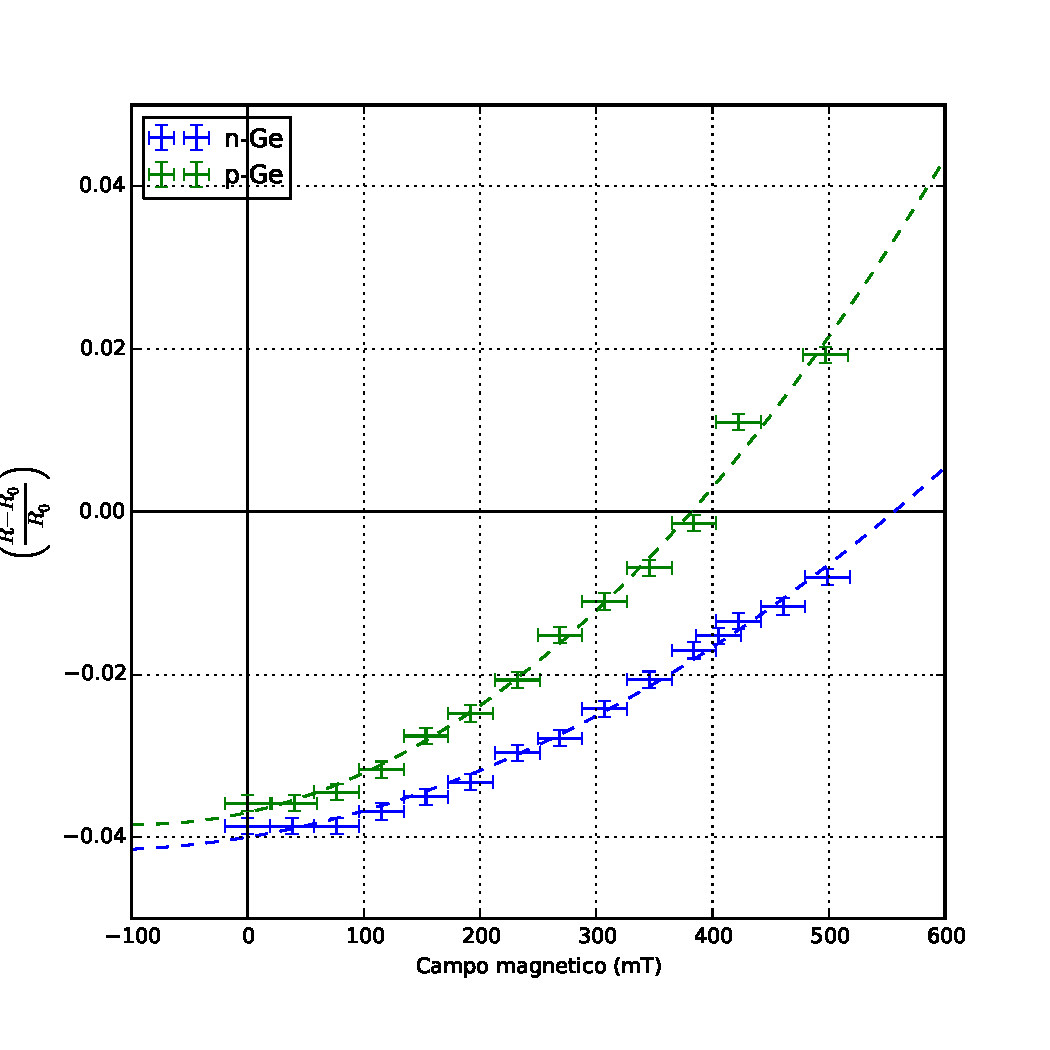
\includegraphics[width=0.45\textwidth]{RMag.pdf}
			\caption{Cambio en la resistencia en función del campo magnético}
			\label{fig:RMag}
		\end{figure}
		
		Se encontró mediante ajustes de los datos que las resistencias siguen la formula
		
	\begin{equation}
		\frac{R-R_0}{R_0}=8.69\times 10^{-8}(mT)^{-2}B^2 + 2.36\times 10^{-05}(mT)^{-1}B - 0.04				
	\end{equation}				

para el tipo n y 

	\begin{equation}
		\frac{R-R_0}{R_0}=1.70\times 10^{-7}(mT)^{-2}B^2 + 3.15\times 10^{-05}(mT)^{-1}B - 0.04		
	\end{equation}		

		para tipo p.
		
		Según la guía de laboratorio, la resistencia debe aumentar con el campo magnético, por lo que actualmente se desconoce el motivo por el cual la mayoría de datos muestran una resistencia decreciente, que sólo empieza a ser positiva para campor magnéticos fuertes. Esto puede deberse al grosor de las muestras, o al hecho de que el campo magnético utilizado estaba en la dirección incorrecta, como se mencionó en la sección \ref{subsec:VHallIConst}. Sin embargo, como se puede observar en el informe \cite{bib:Purwar}, este fenómeno es común para campos magnéticos bajos. En el caso del informe referenciado, antes de 250mT se observó un decrecimiento en la resistencia. Por lo tanto, se puede esperar que a campos magnéticos mayores las regresiones encontradas sigan siendo validas y se observe el aumento en la resistencia. 
		
	\subsection{Conductividad en función de la temperatura}
	
		Lamentablemente, en esta medida se perdieron los datos correspondientes al germanio tipo $p$, y no se pudieron recuperar. La conductividad del germanio tipo $n$ en función de la temperatura es:
		
		\begin{figure}[H]
			\centering
			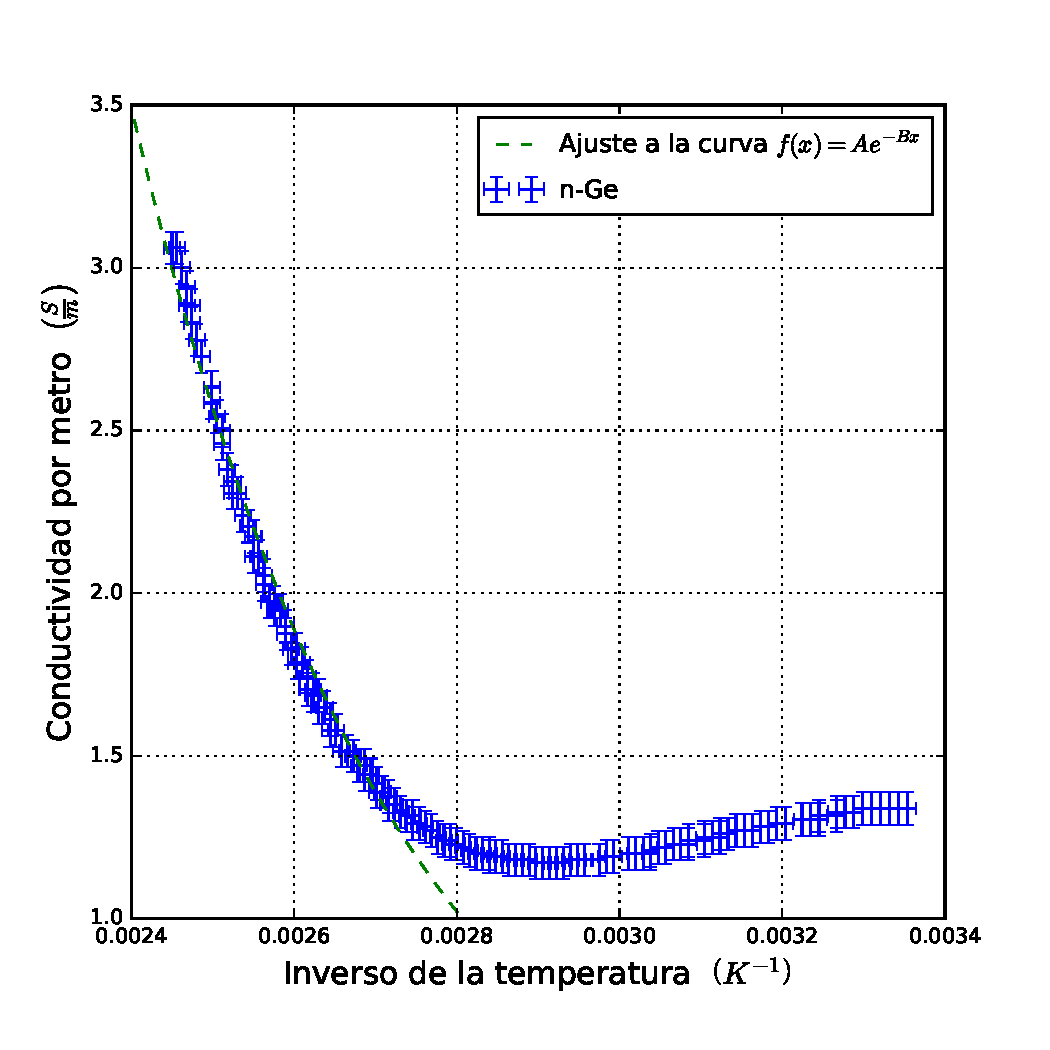
\includegraphics[width=0.45\textwidth]{ConductividadTemp.pdf}
			\caption{Conductividad en función de la temperatura de la muestra}
			\label{fig:CTemp}
		\end{figure}
		
		Los datos que actuaban de la manera más similar a la forma de la ecuación \eqref{eq:CondTemp} se tomaron como parte de la región de conducción intrínseca del material y se utilizaron para determinar que $E_g$ tiene un valor de $0.265\pm 0.005 \ eV$, el cual tiene un error relativo a la literatura\cite{bib:soporteN} del 47.2\%. Esta diferencia puede deberse a factores como desgaste de la muestra, o un error sistemático en la medición. Sin embargo, con los resultados del coeficiente de Hall $R_H$ se determinó que el dopaje de nuestras muestras es muy distinto al de las del reporte en \cite{bib:soporteN}. Ya que el gap de energía depende fuertemente de las características del dopaje, no es extraño que el valor obtenido haya sido distinto.
		
\section{\label{sec:conc} Conclusiones}

\begin{itemize}

\item Se logró observar la dependencia lineal entre campo magnético y corriente de un sistema de bobinas. También se observaron los efectos de la histéresis magnética de un sistema mediante la diferencia entre el campo magnético observado en una región sin semiconductor y con semiconductor.

\item Se determinó la naturaleza de los portadores de distintas muestras de Ge con distintos dopajes. En particular, se evidencio que el coeficiente de Hall es sensible al signo de la carga de los portadores como se predijo en la ecuación \eqref{eq:RH}. 

\item Comparando la distribución de resultados para el coeficiente de Hall obtenido mediante mediciones a campo magnético constante y a corriente constante, se determinó que las mediciones a campo magnético constante son un mejor método para la medición de esta constante. En particular, este método parece no sufrir tantos percances debido a efectos de segundo orden como el efecto de Righi-Leduc o el efecto de Nernst-Ettingshausen.

\item Se determinó que las muestras tipo n y tipo p tienen resistencias de $37\Omega$ y $48\Omega$ respectivamente. Se evidenció el fenómeno de magnetoresistencia con el cambio cuadrático de estas resistencias con el campo magnético. Se observó el fenómeno de decrecimiento de la resistencia con campos magnéticos bajos confirmando las observaciones previas de Purwar en \cite{bib:Purwar}.

\item Analizando el comportamiento de la conductividad con la temperatura bajo la asunción de conductividad intrínseca se obtuvo que la muestra tipo n tiene un gap de energía de $0.265\pm0.005eV$. Este valor difirió fuertemente del valor reportado en la literatura debido a las características del dopaje que invalidan la asunción de conductividad intrínseca. En efecto el valor es evidencia de la utilidad del dopaje para disminuir el gap de energía en superconductores.

\end{itemize}


\begin{thebibliography}{99}

\bibitem{bib:Ge} New Semiconductor Materials. Characteristics and Properties. \textit{Ge-Germanium}[en linea] Recuperado el 12 de Septiembre de 2016 de \url{http://www.ioffe.ru/SVA/NSM/Semicond/Ge/bandstr.html}

\bibitem{bib:tipon} Sasmita. (2015). What do you understand by Intrinsic Semiconductor and Extrinsic Semiconductor? Electronics Post. Recuperado de \url{http://electronicspost.com/what-do-you-understand-by-intrinsic-semiconductor\\-and-extrinsic-semiconductor/}

\bibitem{bib:guia} Laboratorio Intermedio. \textit{Efecto Hall}. \url{https://sicuaplus.uniandes.edu.co/bbcswebdav/pid-1564409-dt-content-rid-16324935_1/courses/201620_FISI2051_01/hall%20%283\%29.pdf}
	
\bibitem{bib:soporteN} PHYWE Systeme GmbH \& Co. (n.d.) \textit{Hall Effect in n-germanium.}

\bibitem{bib:Purwar} Indian Institute of Science Education and Research (2010). Magneto-resistance in Semi-Conductors. Recuperado de \url{https://www.scribd.com/doc/31246090/Magneto-Resistance-in-Semi-conductors}

\end{thebibliography}

\end{document}